\documentclass[12pt]{article}
\usepackage{amsmath, amsfonts, amsthm, amssymb}
\usepackage{fullpage}
\usepackage{enumerate}
\usepackage{hyperref}
\usepackage{multirow}

% For figures
\usepackage{graphicx}
\usepackage{subcaption}

% For code
\usepackage{listings}
% \renewcommand{\cftsecfont}{\rmfamily\mdseries\upshape}
% \renewcommand{\cftsecpagefont}{\rmfamily\mdseries\upshape} % No bold!
 \lstset{ 
  language=R,                     % the language of the code
  basicstyle=\footnotesize\ttfamily, % the size of the fonts that are used for the code
  numbers=none,                   % where to put the line-numbers
  backgroundcolor=\color{white},  % choose the background color. You must add \usepackage{color}
  showspaces=false,               % show spaces adding particular underscores
  showstringspaces=false,         % underline spaces within strings
  showtabs=false,                 % show tabs within strings adding particular underscores
  frame=single,                   % adds a frame around the code
  rulecolor=\color{black},        % if not set, the frame-color may be changed on line-breaks within not-black text (e.g. commens (green here))
  tabsize=2,                      % sets default tabsize to 2 spaces
  captionpos=b,                   % sets the caption-position to bottom
  breaklines=true,                % sets automatic line breaking
  breakatwhitespace=false,        % sets if automatic breaks should only happen at whitespace
  keywordstyle=\color{blue},      % keyword style
  commentstyle=\color{green},   % comment style
  stringstyle=\color{red}      % string literal style
} 

%%%%%%%%%%%%%%%%%%%%CONTENT MACROS%%%%%%%%%%%%%%%%%%%%%%%%%
\renewcommand{\qed}{\quad \ensuremath{\blacksquare}}    % QED blacksquare
\newcommand{\inv}{^{-1}}                            % inverse operator
\newcommand{\sminus}{\backslash}                    % set minus
\newcommand{\N}{\mathbb{N}}                         % natural numbers
\newcommand{\R}{\mathbb{R}}                         % real numbers
\newcommand{\pow}{\mathcal{P}}                      % power set
\newcommand{\Se}{\mathcal{S}}                       % partition
\newcommand{\D}{\mathcal{D}}                        % partition
\newcommand{\e}{\varepsilon}                        % \varepsilon
\renewcommand{\d}{\delta}                           % \delta
\newcommand{\X}{\mathcal{X}}                        % X domain
\newcommand{\Y}{\mathcal{Y}}                        % Y domain
\newcommand{\Z}{\mathcal{Z}}                        % Z domain
\newcommand{\A}{\mathcal{A}}                        % sub-domain
\newcommand{\E}{\mathbb{E}}                         % expected value
\newcommand{\V}{\mathbb{V}}                         % variance
\newcommand{\pr}{\mathbb{P}}                        % probability
\newcommand{\hP}{{\hat P}}                          % 
\newcommand{\cpest}{\widehat{p}_h}                  % clipped estimated density
\newcommand{\cqest}{\widehat{q}_h}                  % clipped estimated density
\newcommand{\pest}{\widetilde{p}_h}                 % estimated density
\newcommand{\qest}{\widetilde{q}_h}                 % estimated density
\newcommand{\dist}{\operatorname{dist}}             % distance operator
\newcommand{\acro}[1]{\textsc{\MakeLowercase{#1}}}
\newcommand{\ol}{\overline}
\renewcommand{\hat}{\widehat}
%%%%%%%%%%%%%%%%%%%%%%%%%%%%%%%%%%%%%%%%%%%%%%%%%%%%%%%%%%%

\renewcommand{\thesubsection}{\arabic{subsection}}

\usepackage{natbib}
\usepackage[disable]{todonotes}

\begin{document}
\begin{center}
{\bf\Large 37-462/662 HW 04 Solutions}\\
Bryan Hooi \& Shashank Singh\\
\end{center}


\subsection*{Problem 1}
See Figure \ref{fig:p1} for a visualization of our clustering, and see the
Appendix for our R code.
%%% BEGIN FIGURE %%%
\begin{figure}[h!]
\centering
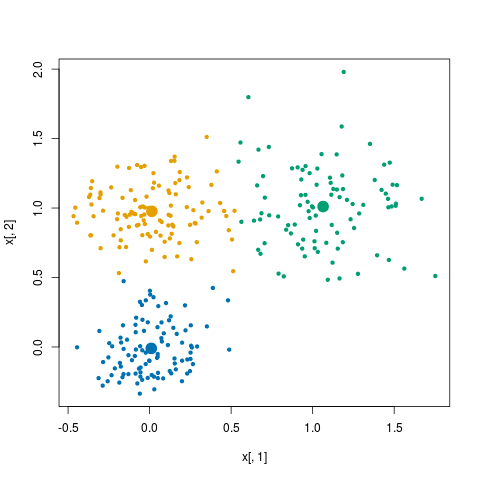
\includegraphics[width=0.8\textwidth]{p1}
\vspace{-2mm}
\caption{Data points and cluster centers, colored by cluster as determined by
$K$-means.}
\label{fig:p1}
\end{figure}
%%% END FIGURE %%%

\newpage
\subsection*{Problem 2}
Calling \texttt{table(km\$cluster, y)} after running \texttt{cancer\_cluster.R}
produces one of the following (depending on the random initialization of
cluster centers:
\begin{verbatim}
           y                                     y
            benign malignant                      benign malignant
          1      9       221                    1    435        18
          2    435        18                    2      9       221
\end{verbatim}
In the first case, cluster 1 consists of mostly malignant tumors and cluster 2
consists of mostly benign tumors; in the second case, the reverse is true. In
either case, we would correctly classify $435 + 221 = 656$ tumors and
incorrectly classify $9 + 18 = 27$ tumors, for a reasonably low
misclassification rate of $0.04\%$. That is, $K$-means recovers the two groups
relatively well.

\subsection*{Problem 3}
\begin{enumerate}[(a)]
\item 
\begin{enumerate}[1.]
\item The cross validated error is $0.0769$.
\item The test error is $0.078$. The values are close and the cross validated error was a good estimate.
\end{enumerate}
\item
\begin{enumerate}[1.]
\item The Out Of Bag (OOB) error is $0.048$. 
\item The test error is $0.042$. 
\item Yes, the OOB error was a good estimate of test error.
\item The random forest has lower test error, and its cross validated error is lower than the random forest OOB error. Yes, if we used cross validation / OOB error we would have chosen the random forest model.
\end{enumerate}
\item
\begin{enumerate}[1.]
\item The 7 most important variables are char\_freq\_exc, char\_freq\_dollar, word\_freq\_remove, word\_freq\_free, capital\_run\_length\_average, word\_freq\_your, capital\_run\_length\_longest.\\
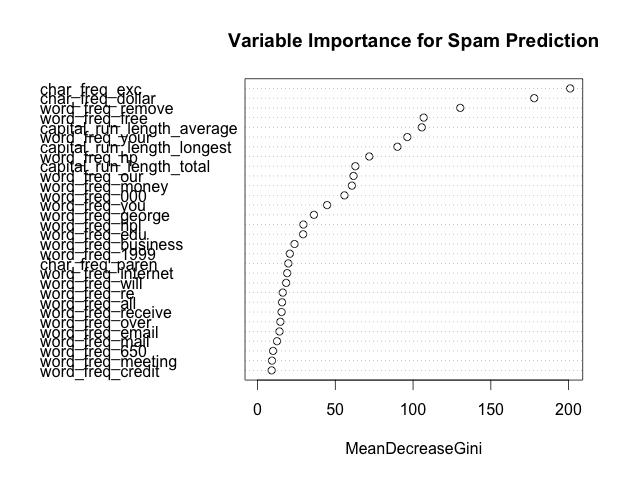
\includegraphics[width=0.5\textwidth]{varImp.png}
\item The probability of being spam increases sharply when word\_freq\_free increases to 1, then remains more or less fixed. The probability of being spam generally decreases as word\_freq\_hp, levelling off when word\_freq\_hp reaches 5. Since both relationships are highly nonlinear, this suggests that linear regression would not be able to capture such trends well.\\
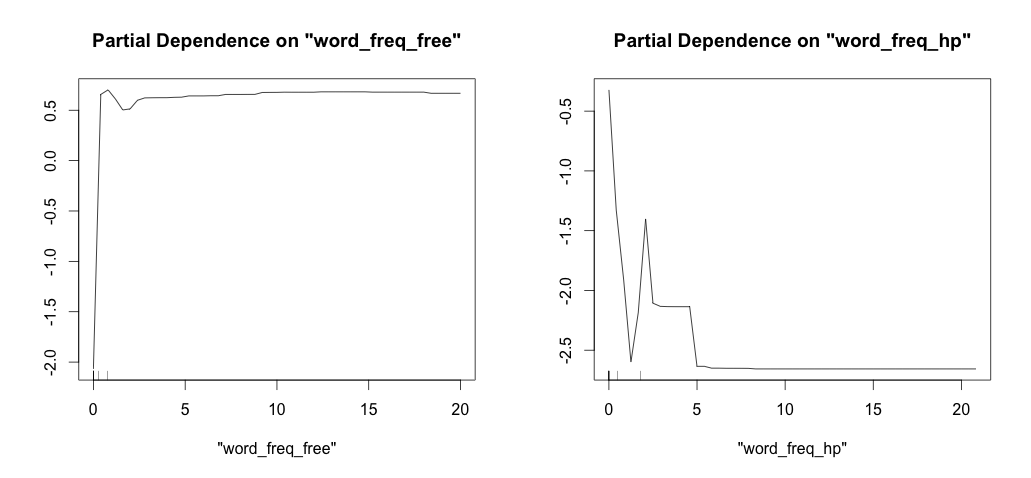
\includegraphics[width=0.9\textwidth]{partialDep.png}
\end{enumerate}
\end{enumerate}

\newpage
\subsection*{Code Appendix}
\subsubsection*{Problem 1}
\begin{lstlisting}
# Arguments:
# x: data matrix, n observations (rows) by p features (cols).
# centers: a vector giving the starting centers. Defaults
#   to NULL in which case we choose k centers at random.
# k: number of clusters. Not needed if centers is specified.
# maxiter: Maximum number of iterations before we quit.  Defaults to 100.
#
# Returns:
# centers: a vector of length k, giving the final centers.
# cluster: a vector of length n, giving the final clustering assignments.
# iter: number of iterations performed.

my.kmeans = function(x, centers=NULL, k=NULL, maxiter=20) {
  n = nrow(x)
  p = ncol(x)
  # Initialize the centers, unless there were supplied in the function call
  # If centers are not given, k must be specified
  if (is.null(centers)) {
    if (is.null(k)) stop("Either centers or k must be specified.")
    centers = matrix(runif(k*p, min(x), max(x)), nrow=k)
  }
  #We can get k from the number of centers we were given
  k = nrow(centers)
  
  cluster = matrix(0, nrow=0, ncol=n)
  cluster.old = cluster
  
  for (iter in 1:maxiter) {
    # Assign each data point to the nearest cluster
    # (we represent assigning data point i to cluster j by cluster[i] = j)
    dists = numeric(k)
    for (i in 1:n) {
      for (j in 1:k) {
        # compute distance from i^th data point to j^th center
        dists[j] = dist(rbind(x[i,], centers[j,])) 
      }

      # assign points to the center with minimum distance
      cluster[i] = which.min(dists)
    }

    # Now that we've computed the cluster assignments, update the centers
    for (j in 1:k) {
      centers[j,] = colMeans(x[cluster == j,])
    }
    
    # If no cluster assignments have changed, we're done.
    if (iter > 1 & all(cluster == cluster.old)) {
      break
    }
    
    cluster.old=cluster # Retain previous clustering to see if it changed
  }
  return(list(centers=centers,cluster=cluster,iter=iter))
}

# Simple test example:
set.seed(0)
x = rbind(matrix(rnorm(2*100,sd=0.2),ncol=2),
          scale(matrix(rnorm(2*100,sd=0.3), ncol=2), cent=-c(1,1), scal=F),
          scale(matrix(rnorm(2*100,sd=0.2), ncol=2), cent=-c(0,1), scal=F))

cent.init = rbind(c(0.5,1),c(1,0),c(0,0.5)) # Initialize the centers

km_yours = my.kmeans(x, centers=cent.init, maxiter=20)
km_truth = kmeans(x, centers=cent.init, iter.max = 20, algorithm = "Lloyd")

# Plot your success!
nicecolors = c("#E69F00", "#009E73", "#0072B2", "#CC79A7")
plot(x[,1], x[,2], pch=20, col=nicecolors[km_yours$cluster])
points(km_yours$centers, pch=20, cex=3, col=nicecolors)
\end{lstlisting}

\newpage
\subsubsection*{Problem 2}
\begin{lstlisting}
#Clear the workspace
rm(list=ls())
set.seed(0)

# Load the data.  NAs are coded as "?"
dat = read.csv('breast-cancer-wisconsin.data', header=FALSE, na.strings="?")
# Label the data fields.  Description and values are as noted.
names(dat) = c(
  'id',# Sample code number            id number
  'thickness',# Clump Thickness               1 - 10
  'size_uniformity',# Uniformity of Cell Size       1 - 10
  'shape_uniformity',# Uniformity of Cell Shape      1 - 10
  'adhesion',# Marginal Adhesion             1 - 10
  'size',# Single Epithelial Cell Size   1 - 10
  'nuclei',# Bare Nuclei                   1 - 10
  'chromatin',# Bland Chromatin               1 - 10
  'nucleoli',# Normal Nucleoli               1 - 10
  'mitoses',# Mitoses                       1 - 10
  'class'# Class:            (2 for benign, 4 for malignant)
  )
dat = dat[,-1] # Drop ID number, we don't want to use this for anything

# Make outcome descriptive
dat$class = ifelse(dat$class==2, "benign", "malignant")

dat$class = as.factor(dat$class) # Make outcome a factor

dat = dat[complete.cases(dat),] # Drop examples with missing data

X = dat[,1:9] # Tumor characteristics
y = dat[,10] # Tumor class

# Cluster the tumors based on X
km = kmeans(X, centers = 2, iter.max = 20, nstart = 10, algorithm = "Lloyd")
# Compare the cluster assignments to y
print(table(km$cluster, y))
\end{lstlisting}

\newpage
\subsubsection*{Problem 3}
\begin{lstlisting}
rm(list=ls())
library(ElemStatLearn)
colnames(spam)[1:57] <- c("word_freq_make", "word_freq_address", "word_freq_all", "word_freq_3d", "word_freq_our", "word_freq_over", "word_freq_remove", "word_freq_internet", "word_freq_order", "word_freq_mail", "word_freq_receive", "word_freq_will", "word_freq_people", "word_freq_report", "word_freq_addresses", "word_freq_free", "word_freq_business", "word_freq_email", "word_freq_you", "word_freq_credit", "word_freq_your", "word_freq_font", "word_freq_000", "word_freq_money", "word_freq_hp", "word_freq_hpl", "word_freq_george", "word_freq_650", "word_freq_lab", "word_freq_labs", "word_freq_telnet", "word_freq_857", "word_freq_data", "word_freq_415", "word_freq_85", "word_freq_technology", "word_freq_1999", "word_freq_parts", "word_freq_pm", "word_freq_direct", "word_freq_cs", "word_freq_meeting", "word_freq_original", "word_freq_project", "word_freq_re", "word_freq_edu", "word_freq_table", "word_freq_conference", "char_freq_semicol", "char_freq_paren", "char_freq_bracket", "char_freq_exc", "char_freq_dollar", "char_freq_pound", "capital_run_length_average", "capital_run_length_longest", "capital_run_length_total")
set.seed(123)  # There's some randomness to rf's
idx = sample(1:nrow(spam),1000,replace=FALSE)
test = spam[idx,]
train = spam[-idx,]

#(a)
library(glmnet)
spam.idx = which(names(train) == "spam")
cv.lasso = cv.glmnet(as.matrix(train[,-spam.idx]), train[,spam.idx], family='binomial', alpha=1, type.measure="class")
cv.err = cv.lasso$cvm[cv.lasso$lambda == cv.lasso$lambda.1se]
pred = predict(cv.lasso, newx=as.matrix(test[,-spam.idx]), s=cv.lasso$lambda.1se, type="class")
test.err = mean(pred != test[,spam.idx])
cat(sprintf("cv error is %f, actual error is %f", cv.err, test.err))
#(b)
library(randomForest)
rf.model = randomForest(spam~., train)
rf.model
pred = predict(rf.model, newdata=test)
test.err = mean(pred != test$spam)
test.err
#(c)
varImpPlot(rf.model, main="Variable Importance for Spam Prediction")
par(mfrow=c(1,2))
partialPlot(rf.model, pred.data=train, "word_freq_free", which.class="spam")
partialPlot(rf.model, pred.data=train, "word_freq_hp", which.class="spam")
\end{lstlisting}


%{\small
%\bibliography{biblio}
%%\bibliographystyle{icml2014}
%\bibliographystyle{plain}
%}
\end{document}
